\documentclass{article}

\usepackage[fleqn]{amsmath}
\usepackage{amssymb}
\usepackage{hyperref}
\usepackage{url}
\usepackage{graphicx}
\usepackage{geometry}
\usepackage[italian]{babel}
\usepackage{enumitem}
\usepackage{parskip}
\usepackage{pgfplots}
\pgfplotsset{compat=1.17}
\usepackage{tikz}
\usetikzlibrary{decorations.text}
\usetikzlibrary{arrows}
\usetikzlibrary{shapes}
\newcommand*\circled[1]{\tikz[baseline=(char.base)]{
            \node[shape=circle,draw,inner sep=1.2pt] (char) {#1};}
}

\geometry{
    a4paper,
    total={170mm, 257mm},
    left=20mm,
    top=20mm
}

\begin{document}

\title{\textbf{Corso passerella \\ Esame di fisica 2022}}
\author{Matteo Frongillo}

\maketitle
\section*{\centering Materiale ammesso}
\begin{enumerate}[label=\textbf{\alph*)}]
    \item \textbf{Materiale personale} \\ Ogni studente può avere:
\end{enumerate}
\begin{enumerate}[label=\textbf{\roman*)}, leftmargin=1.5cm]
    \item del materiale per scrivere e disegnare (penna, matita, gomma, riga, squadra, goniometro, compasso);
    \item una calcolatrice non grafica;
    \item il formulario ufficiale: \textit{Formulari e tavole}.
\end{enumerate}
\begin{enumerate}[label=\textbf{\alph*)}, start=2]
    \item \textbf{Materiale fornito appositamente per l'esame} \\
        Ogni studente riceve:
\end{enumerate}
\begin{enumerate}[label=\textbf{\roman*)}, leftmargin=1.5cm]
    \item il testo dell'esame;
    \item alcuni fogli timbrati da usare per redigere le soluzioni da consegnare e la brutta copia.
\end{enumerate}

\section* {\centering {Indicazioni concernenti il punteggio}}

\begin{enumerate}[label=\textbf{\alph*)}]
    \item Per ogni esercizio è indicato il punteggio
        massimo complessivo, ossia quello ottenuto \\ qualora l'esercizio
        sia svolto completamente e correttamente;
    \item La parte di \textit{fisica} vale un terzo dell'esame di \textit{Scienze sperimentali}.
\end{enumerate}

\pagebreak

\section*{Esercizio 1 - \textit{Circuito con resistori}}
\vspace{-3mm} {\textit{Punteggio complessivo: \textbf{11 punti}}} \vspace{5mm} \\
Considera il circuito nella figura, costituito da una batteria da 120 V
e cinque resistori collegati da cavi di rame (di resistenza trascurabile). \\
Le resistenze valgono: ${R_1} = 20.0$ $\Omega$, ${R_2} = 15.0$ $\Omega$, 
${R_3} = 10.0$ $\Omega$, ${R_4} = 30.0$ $\Omega$, ${R_5} = 25.0$ $\Omega$.

\vspace{1cm}
\begin{figure}[h]
    \centering
    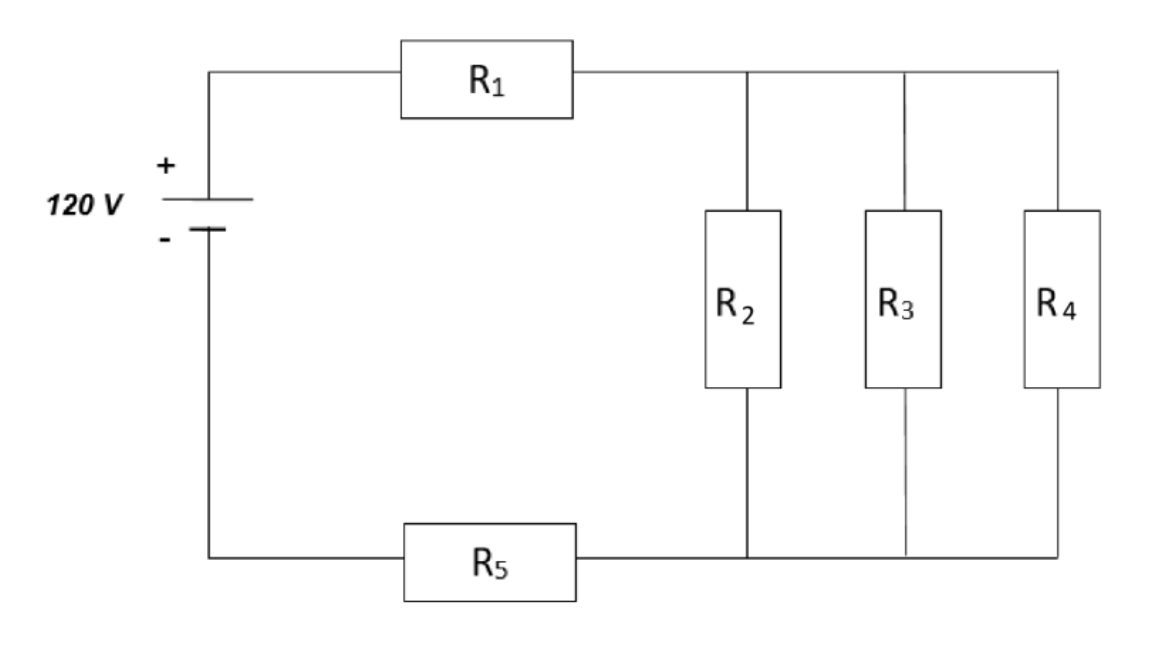
\includegraphics[width=0.9\textwidth]{Esercizio 1.png}
\end{figure}
\vspace{1cm}

\begin{enumerate}[label=\textbf{\alph*)}]
    \item Determina la resistenza equivalente dell'intero circuito.
    \item Dimostra che la corrente che attraversa il resistore $R_1$ vale 2.40 A.
    \item Determina l'intensità della corrente che attraversa il resistore $R_4$.
    \item Determina la differenza di potenziale elettrico ai capi del resistore $R_5$.
    \item Stabilisci quale dei cinque resistori dissipa la maggior potenza e
        determina tale \\ potenza.
    \item Determina il numero di singoli elettroni che ``entrano'' (ed ``escono")
        dal resistore \\ $R_2$ in 5.00 s.
\end{enumerate}

\pagebreak


\section*{Esercizio 2 - \textit{Ciclo termodinamico}}
\vspace{-3mm} {\textit{Punteggio complessivo: \textbf{12 punti}}} \vspace{5mm} \\
Una determinata quantità di gas perfetto (o ideale) viene sottoposta ad una serie 
di trasformazioni che costituiscono un ciclo termodinamico. Si considerino le 
seguenti descrizioni delle trasformazioni e si risponda alle domande poste.

\begin{enumerate}[label=\textbf{\alph*)}]
    \item Il gas si trova inizialmente nello stato $A$, nel quale si occupa un
        volume $V_A = 8.00 \cdot 10^{-3}$ m$^3$ alla temperatura
        $T_A = 300$ K e alla pressione $p_A = 3.00 \cdot 10^5$ Pa.
\end{enumerate}
\begin{enumerate}[label=\textbf{\roman*)}, leftmargin=1.5cm]
    \item Il gas viene portato nello stato $B$, mantenendo la pressione
        costante e raddoppiando il volume. \\
        Determinare la temperatura $T_B$ raggiunta dal gas nello stato $B$
    \item Il gas viene in seguito portato nello stato $C$, mantenendo sempre
        la temperatura costante e riducendo la pressione a 2/3 di
        quella nello stato $B$. \\
        Determinare il volume $V_C$ raggiunto dal gas nello stato $C$.
    \item Mantenendo il volume costante, la pressione viene abbassata fino a 
        raggiungere lo stato $D$, nel quale il gas assume nuovamente la
        temperatura $T_A$ che aveva inizialmente. \\
        Determinare la pressione $P_D$ raggiunta dal gas nello stato $D$
    \item Il gas viene, infine, riportato nello stato di partenza $A$,
        riducendo il suo volume e \\ aumentando la sua pressione a temperatura
        $T_D = T_A$ costante. 
\end{enumerate}
\begin{enumerate}[label=\textbf{\alph*)}, start=2]
    \item Si rappresenti il ciclo, in modo qualitativo ma accurato, 
        ovvero con tutti i dettagli del caso (valori di volume, pressione, 
        temperatura nei quattro stati), nel diagramma $p(V)$ della pagina 
        seguente.
    \item Si risponda inoltre alle seguenti domande a proposito degli scambi
        di energia durante le diverse trasformazioni
\end{enumerate}
\begin{enumerate}[label=\textbf{\roman*)}, leftmargin=1.5cm]
    \item Nel passare dallo stato $A$ allo stato $B$, il gas riceve o cede
        energia sotto forma di lavoro meccanico, rispettivamente sotto
        forma di calore?
    \item Nel passare dallo stato $B$ allo stato $C$, l'energia interna del gas
        aumenta, diminuisce o rimane invariata?
    \item Nel passare dallo stato $C$ allo stato $D$, l'energia interna del gas
        cambia per effetto di uno scambio di lavoro o di calore?
\end{enumerate}
\pagebreak

\begin{figure}[h]
    \begin{center}
        \vspace{4cm}
        {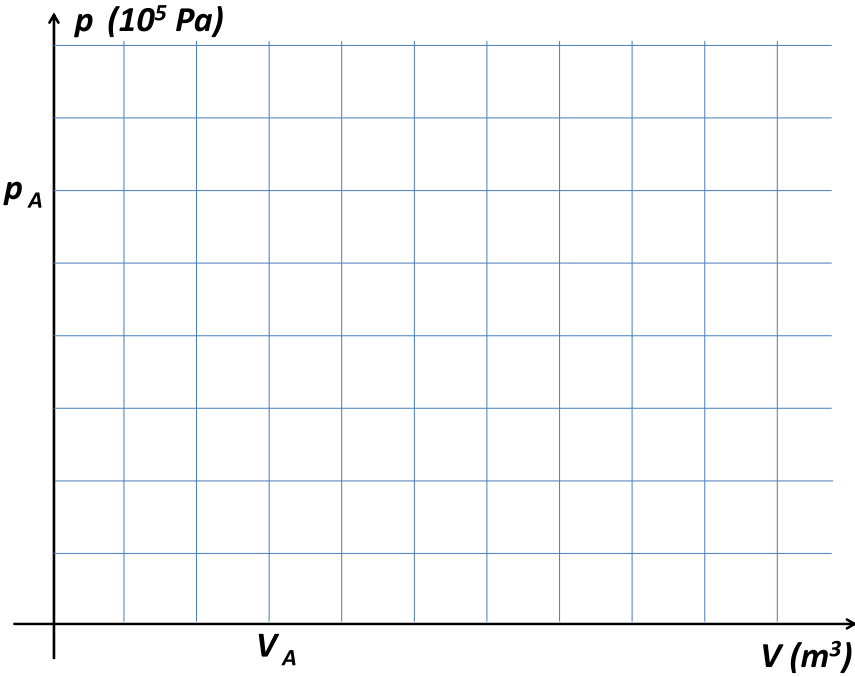
\includegraphics[width=0.9\textwidth]{Esercizio 2.png}}
    \end{center}
\end{figure}
\pagebreak

\section*{Esercizio 3 - \textit{Equilibrio tra forze}}
\vspace{-3mm} {\textit{Punteggio complessivo: \textbf{11 punti}}} \vspace{5mm} \\
Un parallelepipedo rettangolo di massa $M = 200$ g viene appoggiato su di una
molla di massa trascurabile con costante elastica $k = 30.0$ N/m (figura a sinsitra).

\begin{enumerate}[label=\textbf{\alph*)}]
    \item Si rappresentino le forze che agiscono sul parallelepipedo e si 
        calcoli quanto vale la \\ compressione $\Delta{x}$ della molla. 
\end{enumerate}

\begin{figure}[h]
    \centering
    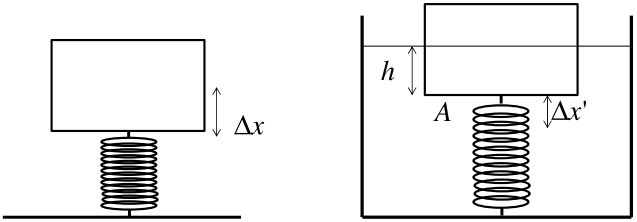
\includegraphics[width=0.8\textwidth]{Esercizio 3.png}
    \vspace{0.4cm}
\end{figure}

Quando si immerge il parallelepipedo poggiato sulla molla in un liquido di
densità $\rho = 870$ kg/m$^3$ (figura a destra), si osserva che galleggia,
restando immerso per $h = 3.00$ cm. Inoltre, a differenza della prima
situazione, ora l'allungamento della molla rispetto alla lunghezza di
riposo è $\Delta{x'}$. \\ Nella nuova situazione:

\begin{enumerate}[label=\textbf{\alph*)}, start=2]
    \item Si disegnino le forze che agiscono sul parallelepipedo;
    \item Si scriva l'equazione di equilibrio delle forze agenti sul parallelepipedo;
    \item Se l'area di base $A$ del parallelepipedo è di 1.20 dm$^2$, si
        determini l'allungamento $\Delta{x'}$
\end{enumerate}
\pagebreak

\section*{Esercizio 4 - \textit{Un carrello}}
\vspace{-3mm} {\textit{Punteggio complessivo: \textbf{12 punti}}} \vspace{5mm} \\
Una molla di costante elastica $k$ è posta, in orizzontale, al termine di un
piano inclinato di 30.0°, sul quale si muove un carrello di massa
$m = 150$ g. Come si vede in figura, il carrello è inizialmente fermo a
un'altezza $h = 30.0$ cm, quando viene liberato (consideralo puntiforme).

\begin{figure*}[h]
    \centering
    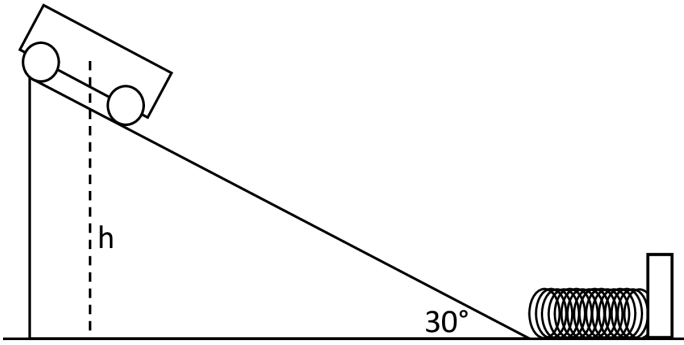
\includegraphics[width=.8\textwidth]{Esercizio 4.png}
    \vspace{0.4cm}
\end{figure*}

\textbf{SITUAZIONE A: trascurando ogni forma di attrito.}
\begin{enumerate}[label=\textbf{\alph*)}]
    \item Calcola l'intensità della forza normale del piano sul carrello;
    \item Calcola la velocità del carrello quando arriva sulla molla;
    \item Determina l'altezza massima $h'$ raggiunta dal carrello
    risalendo sul piano dopo il rimbalzo sulla molla.
        \linebreak
        \linebreak
        A seguito dell'impatto con il carrello, la molla raggiunge una
        compressione massima di $\Delta{x} = 2.50$ cm:
    \item Quanto vale l'energia potenziale elastica immagazzinata
        dalla molla?
    \item Calcola la costante elastica $k$ della molla.
\end{enumerate}
\vspace{2.5mm}
\textbf{SITUAZIONE B: con un attrito radente dinamico tra piano e carrello.}
    \\ In presenza di attrito, liberando il carrello sempre dalla quota
    $h = 30.0$ cm, si osserva una compressione massima della molla di
    $\Delta{x'} = 2.00$ cm.
\begin{enumerate}[label=\textbf{\alph*)}]
    \item Determina il coefficiente di attrito dinamico $\mu$ tra
        carrello e piano;
    \item Rappresenta le forze cui è sottoposto il carrello nella risalita
        (una volta abbandonata la molla);
    \item Determina l'altezza massima $h''$ raggiunta dal carrello
        risalendo sul piano dopo il rimbalzo sulla molla.
\end{enumerate}

\pagebreak

\section*{Soluzioni}
\subsection*{Esercizio 1}
\vspace*{1cm}
\begin{enumerate}[label=\textbf{1\alph*)}]
    \item \begin{align*}
        R_{tot} & = R_1 + R_5 + \frac{1}{\frac{1}{R_2}+\frac{1}{R_3}+\frac{1}{R_4}} \\
        & = 20 \Omega + 25 \Omega + 
        \frac{1}{\frac{1}{15\Omega} +\frac{1}{10\Omega} +\frac{1}{30\Omega}} \\
        & = 50 \Omega
    \end{align*}
    \item \begin{align*}
        U & = R \cdot I \Rightarrow I = \frac{U}{R} \\
        I & = \frac{120V}{50\Omega} = 2.4 A
    \end{align*}
    \item \begin{align*}
        I_{R_4} & = \frac{R_2 \parallel R_3}{R_2 \parallel R_3 + R_4} \cdot I_{tot} \\
        \\
        R_2 \parallel R_3 & = \frac{1}{\frac{1}{15\Omega}+\frac{1}{10\Omega}}
        = 6\Omega \\
        \\
        I_{R_4} & = 
        \frac{6\Omega \cdot 2.4 V}{6\Omega + 30\Omega} = 0.4V
    \end{align*}
    \item \begin{align*}
        U &= R \cdot I \\
        U &= 25\Omega \cdot 2.4 A = 60V \\
        &\text{Ponendo } U_0 = 0V \\
        \Delta{U} &= U - U_0 = 60V - 0V = 60V
    \end{align*}
    \item \begin{align*}
        \begin{cases}
            P = U \cdot I \\
            U = R \cdot I 
        \end{cases} \Rightarrow P &= R \cdot I^2 \\
        P_5 &= 25\Omega \cdot (2.4A)^2 = 144 W
    \end{align*}
    \item \begin{align*}
        N_{e^-} &= \left\lvert\frac{I \cdot t}{\text{Carica elettrica }e^-}\right\rvert \\
        N_{e^-} &= \left\lvert\frac{2.4A \cdot 5s}{-1.602 \cdot 10^{-19} C}\right\rvert
        \thickapprox 7.5 \cdot 10^{19} \text{ elettroni}
    \end{align*}
\end{enumerate}
\pagebreak

\subsection*{Esercizio 2}
\textbf{2a)} \\

\hspace*{0.85cm}\textbf{LEGGE DEI GAS PV=nRT} \\
\begin{equation*}
   nR = costante \Rightarrow \frac{V_i \cdot p_i}{T_i} = \frac{V_f \cdot p_f}{T_f} 
\end{equation*} \\

\begin{enumerate}[label=\textbf{.\roman*)}]
    \item \begin{align*}
        &\circled{A} \begin{cases}
            V_A = 8 \cdot 10^{-3}\ m^3 \\
            p_A = 3\cdot 10^5\ Pa \\
            T_A = 300\ K
        \end{cases} \\ \\
        &\circled{A} \Rightarrow \circled{B} \\ \\
            &\frac{V_A \cdot p_A}{T_A} = \frac{2V_A \cdot p_A}{T_B}
            \Rightarrow T_B = \frac{T_A}{V_A} \cdot 2V_A
            \Rightarrow T_B = \frac{300\ K}{8\cdot10^{-3}\ m^3} \cdot 16\cdot10^{-3}\ m^3
            \Rightarrow T_B = 600\ K
    \end{align*}
    \item \begin{align*}
        &\circled{B} \Rightarrow \circled{C} \\ \\
        &\frac{2V_A \cdot p_A}{T_B} = \frac{V_C\cdot2p_A}{3T_B}
        \Rightarrow V_C = \frac{2V_A \cdot 3p_A}{2p_A}
        \Rightarrow V_C = \frac{16\cdot10^{-3}\ m^3 \cdot 3(3\cdot10^5)\ Pa}{2(3\cdot10^5)\ Pa}
        \Rightarrow V_C = 0.024\ m^3
    \end{align*}
    \item \begin{align*}
        &\circled{C} \Rightarrow \circled{D} \\ \\
        &\frac{V_C \cdot 2p_A}{3T_B} = \frac{V_C \cdot p_D}{T_A}
        \Rightarrow p_D = \frac{2p_A \cdot T_A}{3T_B}
        \Rightarrow p_D = \frac{2(3\cdot10^5\ Pa) \cdot 300\ K}{3\cdot 600\ K}
        \Rightarrow p_D = 10^5\ Pa
    \end{align*}
    \item \hspace{0.85cm}$\circled{D} \Rightarrow \circled{A}$
\end{enumerate}
\pagebreak
\textbf{2b)} \\

\begin{figure}[h]
    \centering
    \begin{tikzpicture}
    \begin{axis}[
        title={\textbf{2b} Ciclo di Carnot},
        xlabel={Volume ($10^{-2}\ \text{m}^3$)},
        ylabel={Pressione ($10^5$ Pa)},
        xmin=0, xmax=0.03,
        ymin=80000, ymax=350000,
        xtick={0.008, 0.016, 0.024},
        ytick={100000, 200000, 300000},
        grid style=dashed,
        ]

        % Adding points
        \addplot[
            color=blue,
            mark=*,
            mark size=1.5pt,
            only marks,
            point meta=explicit symbolic,
            nodes near coords,
            visualization depends on={value \thisrow{anchor} \as \myanchor},
            every node near coord/.append style={font=\footnotesize, anchor=\myanchor}
        ] table[meta=label] {
            x       y       label   anchor
            0.008   300000  300K    south
            0.016   300000  600K    south
            0.024   200000  600K    west
            0.024   100000  300K    west
        };
        
        % Connecting points

        \addplot[
            color=red, 
            thick,
            no marks,
            -stealth,
            line width=.3mm
        ] coordinates {
            (0.008, 300000)
            (0.016, 300000)
        };
        \node at (axis cs:0.012, 310000) {\tiny Isobara};

        \addplot[
            color=red,
            thick,
            no marks,
            -stealth,
            line width=.3mm,
            smooth,
            tension=1
        ] coordinates {
            (0.016, 300000)
            (0.018, 235000)
            (0.024, 200000)
        };
        \node at (axis cs:0.020, 250000) {\tiny Isoterma};
        
        \addplot[
            color=red,
            thick,
            no marks,
            -stealth,
            line width=.3mm
        ] coordinates {
            (0.024, 200000)
            (0.024, 100000)
        };
        \node at (axis cs:0.02625, 150000) {\tiny Isocora};
        
        \addplot[
            color=red,
            thick,
            no marks,
            -stealth,
            line width=.3mm,
            smooth,
            tension=1
        ] coordinates {
            (0.024, 100000)
            (0.012, 170000)
            (0.008, 300000)
        };
        \node at (axis cs:0.009, 170000) {\tiny Isoterma};
        
    \end{axis}
    \end{tikzpicture}
\end{figure}

\textbf{2c)} \\

\begin{enumerate}[label=\textbf{.\roman*)}]
    \item Il gas si espande tramite lavoro meccanico, di conseguenza si riscalda.
    \item La temperatura rimane costante e non causa differenze di energia,
        dunque rimane invariata.
    \item La temperatura diminuisce a causa di uno scambio di calore.
\end{enumerate}
\pagebreak

\subsection*{Esercizio 3}

\begin{enumerate}[label=\textbf{3\alph*)}]
    \item $\vec{F}=m\cdot g \Rightarrow F=0.2kg \cdot 9.81 \frac{N}{kg}=1.962N \\ \\
        \Delta x=\frac{F}{k} \Rightarrow \Delta x=\frac{1.962N}{30\frac{N}{m}}
        = 0.0654m = 65.4mm$
    \item \phantom{}
        \begin{figure*}[h!]
            \hspace*{.75cm} \includegraphics*[width=.25\textwidth]{Esercizio 3 - Forze.png}
        \end{figure*}
    \item $\vec{F}_g = \vec{F}_A + \vec{F}_k \Rightarrow m g = \rho g V + k \Delta x' $
    \item $1.962N = 870 \frac{kg}{m^3} \cdot 9.81 \frac{N}{kg} \cdot 0.012 m^2 \cdot 0.03m + 
    30 \frac{N}{m} \cdot \Delta x' \Rightarrow \Delta x' = -0.037m = -3.7cm$\\
    La molla si comprime di 3.7 cm.
\end{enumerate}
\pagebreak

\subsection*{Esercizio 4}
\begin{enumerate}[label=\textbf{4a.\alph*)}]
    \item $\vec{F}_N = m\cdot g\cdot cos(\alpha) \Rightarrow F_N = 0.15kg \cdot 9.81 \frac{N}{kg}
        \cdot cos(30$\textdegree) = 1.28 N
    \item $\frac{v^2}{2}=g\Delta h \Rightarrow v=\sqrt{2gh} =2.4\frac{m}{s}$
    \item $h'= h$\ \textrightarrow\ Non essendoci attrito l'energia cinetica rimane invariata.
    \item $U_K = \frac{k\Delta x^2}{2}=\frac{29.43 \frac{N}{m} \cdot (0.025m)^2}{2} = 9.2 \cdot 10^{-3} J$
    \item $k= \frac{m\cdot g\cdot sin(\alpha)}{\Delta x}=29.43 \frac{N}{m}$
\end{enumerate} \phantom{}\\
\begin{enumerate}[label=\textbf{4b.\alph*)}]
    \item $m\cdot g\cdot sin(\alpha)\cdot \mu = k\Delta x' \Rightarrow
        \mu= \frac{k\Delta x'}{m\cdot g\cdot sin(\alpha)} \Rightarrow
        \mu= \frac{29.43 \frac{N}{m}\cdot 0.02m}{0.74N}=0.8$
    \item TODO
    \item $\frac{k(\Delta x')^2}{2}=mgh'+ \vec{F}_k \Rightarrow
        \frac{k\Delta x'^2}{2}=mgh'+\mu m\cdot g\cdot cos(\alpha)\frac{h'}{sin(\alpha)}\\
        h'=\frac{\frac{1}{2} k\Delta x^2}{mg+\mu \cdot mg \frac{cos(\alpha)}{sin(\alpha)}}
        \Rightarrow h'=1.68*10^{-3}=1.68mm$
\end{enumerate}



\end{document}